\section{Introduction}

Cite example\cite{coflow}.

One figure example Fig. \ref{fig:attributes}.

%begin figure
\begin{figure}[h]
    \centering
    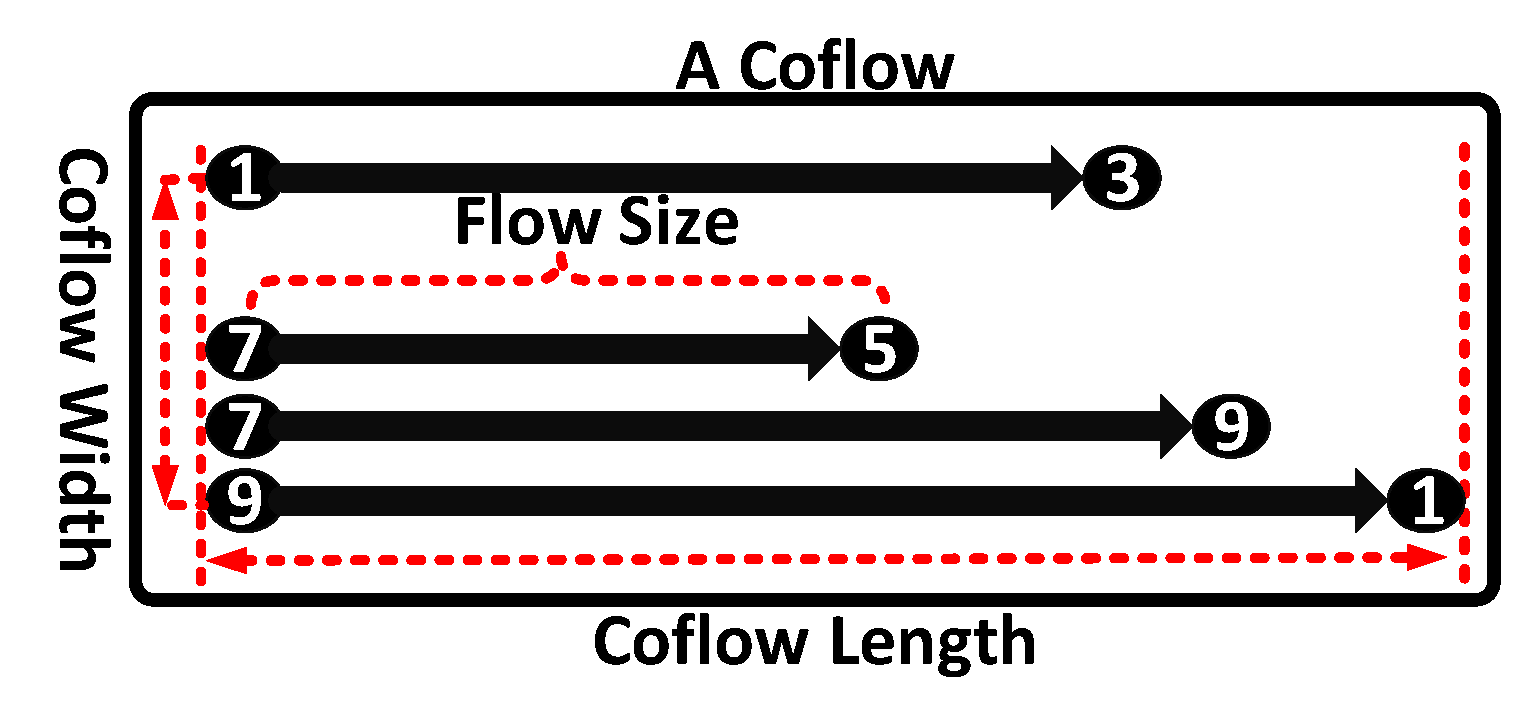
\includegraphics[width=3.2in]{./figures/example/attributes}
    \caption{The attributes of coflows}
    \label{fig:attributes}
\end{figure}
%end Figure
Two figure example, Fig. \ref{fig:m1}.
%begin figure
\begin{figure}[h]
  \centering
  \begin{tabular}[c]{@{}r@{}l@{}}
%  \hline
    \begin{subfigure}[t]{1.6in}
        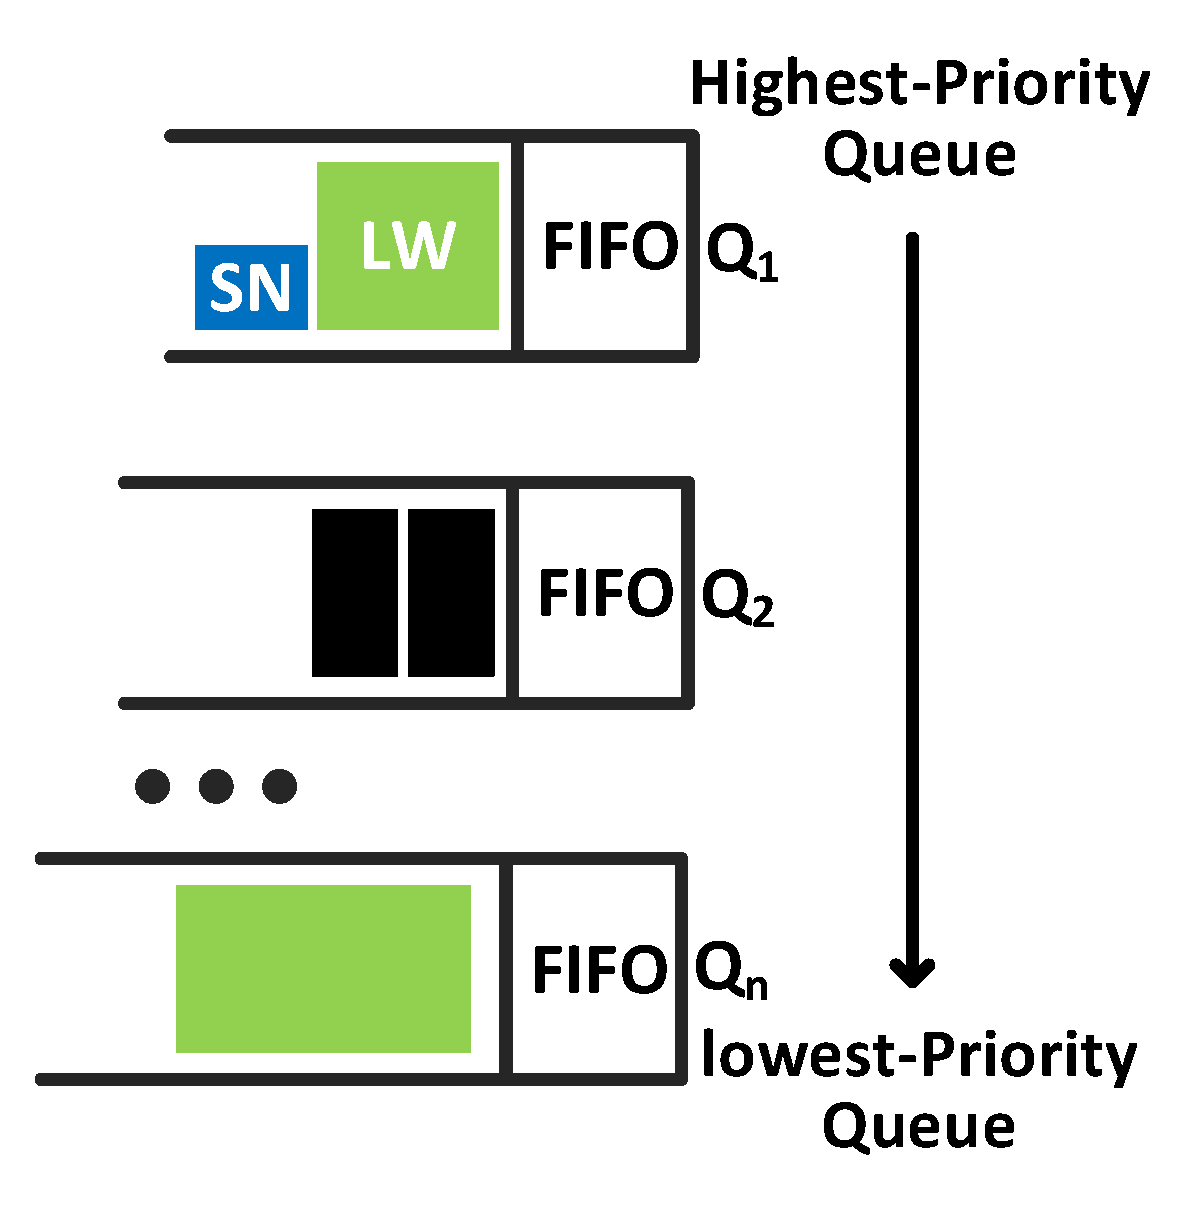
\includegraphics[width=1.6in]{./figures/example//M1a}
        \caption{With the highest priority}\label{fig:m1a}
    \end{subfigure}
    &
    \begin{subfigure}[t]{1.6in}
        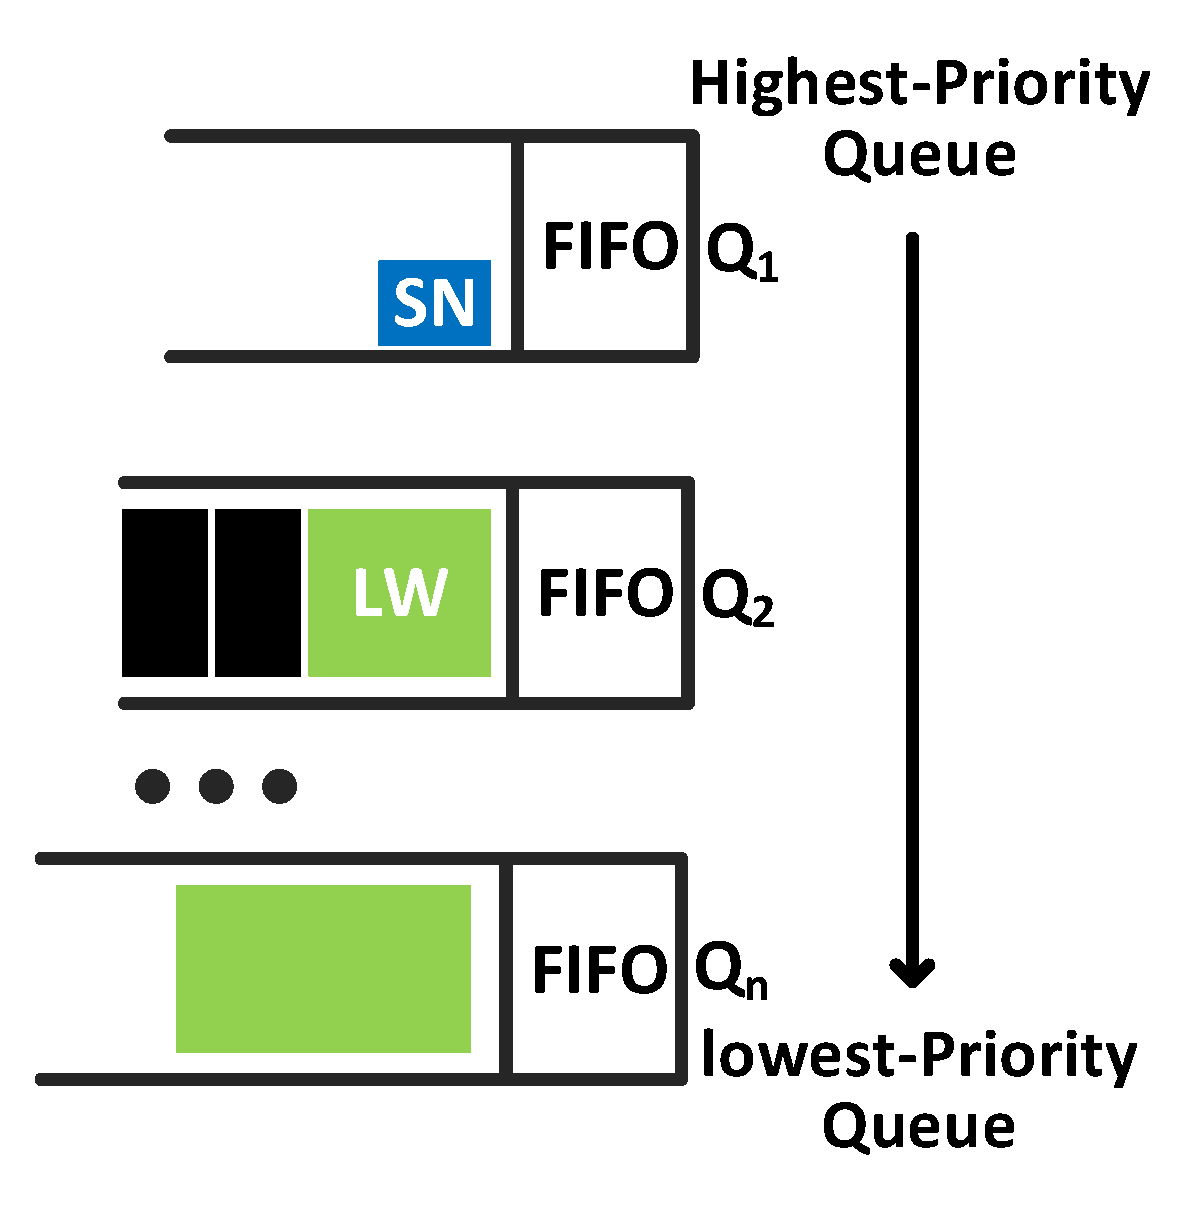
\includegraphics[width=1.6in]{./figures/example/M1b}
        \caption{With different priorities}\label{fig:m1b}
    \end{subfigure}
    \\
%    \hline
  \end{tabular}
  \caption{Impact of HOL blocking. Long-wide coflow $C_1$ in green is scheduled before short-narrow coflow $C_2$ (blue) }\label{fig:m1}
\end{figure}
%end figure

Table example, Table \ref{table:correlation}


\begin{table}[h]
\newcommand{\tabincell}[2]{\begin{tabular}{@{}#1@{}}#2\end{tabular}}
  \centering
  \begin{tabular}[c]{c|c|c|c|c}
      \toprule
      % after \\: \hline or \cline{col1-col2} \cline{col3-col4} ...
      Attributes&\tabincell{c}{Coflow\\Width} &\tabincell{c}{Coflow\\Size}& \tabincell{c}{Minimal\\CCT} &\tabincell{c}{Coflow\\Length}\\
      \midrule
      \tabincell{c}{Coflow\\Width} & 1/1&\tabincell{c}{0.54/0.91\\(0.89,0.92)}& \tabincell{c}{0.5/0.81\\(0.77,0.83)} & \tabincell{c}{0.22/0.37\\(0.29,0.44)}\\
      \hline
      \tabincell{c}{Coflow\\Size} & \tabincell{c}{0.54/0.91\\(0.89,0.92)}& 1/1& \tabincell{c}{0.97/0.96\\(0.96,0.97)} & \tabincell{c}{0.46/0.71\\(0.67,0.75)}\\
      \hline
      \tabincell{c}{Minimal\\CCT} & \tabincell{c}{0.5/0.81\\(0.77,0.83)}& \tabincell{c}{0.97/0.96\\(0.96,0.97)}& 1/1 & \tabincell{c}{0.51/0.82\\(0.78,0.84)}\\
      \hline
      \tabincell{c}{Coflow\\Length} & \tabincell{c}{0.22/0.37\\(0.29,0.44)}& \tabincell{c}{0.46/0.71\\(0.67,0.75)}& \tabincell{c}{0.51/0.82\\(0.78,0.84)} & 1/1\\
      \bottomrule
   \end{tabular}
   \caption{The Pearson correlation coefficient between different attributes. The values in each box are $\rho_{X,Y}$, $\rho_{\log_{10} X,\log_{10} Y}$ and  (the confidence interval) }\label{table:correlation}
\end{table}

Algorithm example. Algorithm \ref{algo:MCS}

%begin algorithm
\begin{algorithm}
\caption{The Main MCS Algorithm}
\begin{algorithmic}[h]

    \Function {Reschedule}{\textbf{Queues} $Q$}
        \For {$i \in 1...n-1$}
            \For {Coflow $k \in Q_i$}
                \If {$w^{(k)}\leq\Delta_w  \text{ and }  \widetilde{d^{(k)}}>\theta_i^n$}
                    \State Remove $k$ from $Q_i$ and put $k$ into $Q_{i+1}$
                \EndIf
                 \If {$w^{(k)}>\Delta_w  \text{ and }  \widetilde{l^{(k)}}>\theta_i^w$}
                    \State Remove from $Q_i$ and put to $Q_{i+1}$
                \EndIf
            \EndFor
        \EndFor
    \EndFunction

    \Function {NewCoflow}{\textbf{Queues} $Q$, \textbf{Coflow} $k$}
        \For {$i \in 1...n-1$}
            \If {$\Delta_{i-1} \leq w^{(k)}< \Delta_i$}
                \State put $k$ into $Q_{p_i}$
                \State Break
            \EndIf
         \EndFor
    \EndFunction
\end{algorithmic}
\label{algo:MCS}
\end{algorithm}
%end algorithm
Formula example. Equation \ref{equation:subject2}
\begin{align}
\centering
min \quad & \sum_{i=1}^{n}\{\sum_{j=1}^{n}[(F^i(\theta_j^i)-F^i(\theta_{j-1}^{i}))\sum_{l=0}^{j} S_l^i]\}\\
\text{subject to}  \quad & \theta_0^i=0,\theta_j^i=\infty \\
\quad & \theta_{j-1}^i \leq \theta_j^i\label{equation:subject2}
\end{align}